%Optics Homework_1
\documentclass[10pt,a4paper]{article}
\usepackage[UTF8]{ctex}
\usepackage{bm}
\usepackage{amsmath}
\usepackage{extarrows}
\usepackage{amsthm}
\usepackage{amssymb}
\usepackage{graphicx}
\usepackage{multirow}
\title{光学作业\#1}
\author{陈稼霖 \and 45875852}
\date{2018.9.19}
\theoremstyle{remark}
\newtheorem{defi}{Definition}
\newtheorem{cdefi}{\bf 定义}
\begin{document}
\maketitle
\section*{1-1}解:
设地面上能见到日全蚀区域的半径为$r$。根据光的直线传播定律和相似三角形的几何关系,有
\[
\frac{r}{x} = \frac{D_{lunar} / 2}{x + d_{lunar-earth}} = \frac{D_{solar} / 2}{x + d_{solar-earth}}
\]
代入太阳直径$D_{solar} = 1.39\times10^6km$,月球直径$D_{lunar} = 3.5\times10^3km$,太阳到地面的距离为$d_{solar-earth} = 1.50\times10^9km$,月球到地面的距离为$d_{lunar-earth} = 3.8\times10^5km$,解得
\[
r = 1.6\times10^3km
\]
故地面上能见到日全蚀区域的面积为
\[
S = \pi\times r^2 = 7.8\times10^6{km}^2
\]
\section*{1-2}证明:
不妨以隅角棱镜上三个直角三角形公共的顶点为原点,以该点所在的三条棱分别为$x$轴、$y$轴、$z$轴,做空间直角坐标系,设从斜面入射的光线所在的直线方程为
\[
\frac{x - x_0}{a} = \frac{y - y_0}{b} = \frac{z - z_0}{c}
\]
即光线所在直线经过点$N(x_0,y_0,z_0)$,且与向量$\overrightarrow{n} = (a,b,c)$平行。又不妨设该光线先经隅角棱镜在$xOy$平面上的面发生全反射,再经在$yOz$ 平面上的面发生全发射,最后经在$zOx$ 平面上的面发生全反射。当发生第一次反射时,光线所在直线所经点$N$关于反射面(即$xOy$平面)的虚像为$N'(x_0,y_0,-z_0)$,此即第一次反射后光线所在直线将要经过的点,同时,与光线所在直线平行的向量变为$\overrightarrow{n'} = (a,b,-c)$,故光线所在直线的方程变为
\[
\frac{x - x_0}{a} = \frac{y - y_0}{b} = \frac{z - (-z_0)}{-c}
\]
同理,当发生第二次全反射时,光线所在直线的方程变为
\[
\frac{x - (-x_0)}{-a} = \frac{y - y_0}{b} = \frac{z - (-z_0)}{-c}
\]
当发生第三次全反射时,出射光线所在直线的方程为
\[
\frac{x - (-x_0)}{-a} = \frac{y - (-y_0)}{-b} = \frac{z - (-z_0)}{-c}
\]
也可以写成
\[
\frac{x - (x_0)}{a} = \frac{y - (-y_0)}{b} = \frac{z - (-z_0)}{c}
\]
故从入射面射入的光线经其他三面全反射后的出射光线所在的直线经过点$N'''(-x_0,-y_0,-z_0)$,且仍与向量$\overrightarrow{n} = (a,b,c)$平行。出射光线不可能与入射光线同向,否则出射光线将穿透隅角棱镜,这违背光线经三个面发生三次全反射的题设,故出射光线的方向与入射线相反。

其余全反射面顺序不同的情况可以类似推出,得到相同的结果。因此,从入射面射入的光线经其他三面全反射后,出射方向总与入射线相反。

隅角棱镜可以将光线反方向反射,且由于反射过程均为全反射,因此反射过程中损耗很小。鉴于其上述的物理性质,隅角棱镜可以:(1)用作激光干涉仪的反射镜;(2)用作激光测距系统的反射镜——将隅角棱镜放置在需要测距的地点,用激光器向隅角棱镜发射激光并记录时间,接收反射回来的激光并记录时间,可以通过激光发射和接收的时间差计算出激光器坐在地和隅角棱镜所在地之间的距离。在这两种应用中应用隅角棱镜时,不需要精密地调节隅角棱镜的朝向,就可以使入射光原路反射,大大提高可操作性,且可使信号损耗很小。
\section*{1-3}
\subsection*{(1)}证明:
设棱镜相对于空气折射率为$n$。如图\ref{FigureofProblem1-3}做各反、折射面法线并对各角、各交点标号。
在BC折射面上,根据斯涅尔定律,有
\[
\sin\theta_1 = n\sin\theta_2
\]
在四边形$ABEF$中,有
\begin{align*}
&\alpha + \beta + 90^{\circ} + \theta_7 = 360^{\circ}\\
&\Longrightarrow\theta_7 = 270^{\circ} - \alpha - \beta
\end{align*}
在三角形$EFG$中,有
\begin{align*}
&\theta_2 + \theta_7 + \theta_8 = 180^{\circ}\\
&\Longrightarrow\theta_8 = 180^{\circ} - \theta_2 - \theta_7 = \alpha + \beta - \theta_2 - 90^{\circ}
\end{align*}
角$\angle DGE$和角$\angle EGH$互余,有
\[
\theta_3 = 90^{\circ} - \theta_8 = \alpha + \beta - \theta_2 - 90^{\circ}
\]
在四边形$AGHI$中,有
\begin{align*}
&\alpha + \theta_11 + 2\times90^{\circ} = 360^{\circ}\\
&\Longrightarrow\theta_11 = 180^{\circ} - \alpha
\end{align*}
在三角形$GHI$中,有
\begin{align*}
&\theta_3 + \theta_4 + \theta_11 = 180^{\circ}\\
&\Longrightarrow\theta_4 = 180^{\circ} - \theta_3 - \theta_11 = 2\alpha + \beta - \theta_2 - 180^{\circ}
\end{align*}
角$\angle BIJ$和角$\angle HIJ$互余,有
\[
\theta_9 = 90^{\circ} - \theta_4 = 270^{\circ} + \theta_2 - 2\alpha - \beta
\]
在四边形$BCJI$中,有
\begin{align*}
&2\alpha + \beta + \theta_9 + \theta_10 = 360^{\circ}\\
&\Longrightarrow\theta_10 = 360^{\circ} - 2\alpha - \beta - \theta_9 = 90^{\circ} - \theta_2
\end{align*}
角$\theta_5$和角$\theta_10$互补,有
\[
\theta_5 = 90^{\circ} - \theta_10 = \theta_2
\]
在CD折射面上,根据斯涅耳定律,有
\begin{align*}
&n\sin\theta_5 = \sin\theta_6\\
\Longrightarrow\sin\theta_6 = \sin\theta_1
\end{align*}
又角$\theta_1$和角$\theta_6$均为锐角,故
\[
\theta_1 = \theta_6
\]
偏转角
\begin{equation}
\label{DeflectionAngle}
\delta = 2\alpha + \theta_1 - \theta_6 = 2\alpha
\end{equation}
为一与入射角无关的常数。
\begin{figure}[h]
\centering
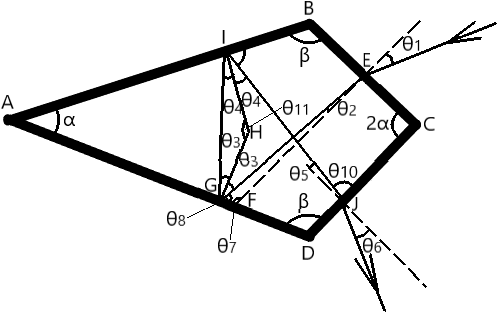
\includegraphics[scale = .8]{FigureofProblem1-3.png}\\
\caption{1-3题图}\label{FigureofProblem1-3}
\end{figure}
\subsection*{(2)}答:
在此条件下,不能产生色散,因为对于不同频率的光,棱镜相对于空气的折射率不同,然而如式\ref{DeflectionAngle}所示,偏转角与棱镜相对于空气的折射率无关,故无法产生色散。
\section*{1-4}证明:
如图\ref{FigureofProblem1-4},设折射角为$\theta'$。根据几何关系,有
\[
AB = \frac{AC}{\cos\angle BAC} = \frac{t}{\cos\theta'}
\]
侧向平移为
\begin{align*}
BD &= AB(\sin\angle CAD - \sin\angle BAC) = \frac{t}{\cos\theta'}\sin(\theta - \theta')\\
&= \frac{t}{\cos\theta'}(\sin\theta\cos\theta' - \cos\theta\sin\theta')\\
&= t(\sin\theta - \frac{\cos\theta\sin\theta'}{\cos\theta'})
\end{align*}
根据斯涅耳定律,有
\[
\sin\theta = n\sin\theta'
\]
由于入射角$\theta$很小且$\theta' < \theta$,故有近似
\begin{align*}
&\sin\theta\approx\theta\\
&\cos\theta\approx\cos\theta'\approx1
\end{align*}
代入可得
\[
\sin\theta'\approx\frac{\theta}{n}
\]
因此,侧向平移为
\[
AB\approx t(\theta - \frac{\theta}{n}) = \frac{n - 1}{n}\theta t
\]
\begin{figure}[h]
\centering
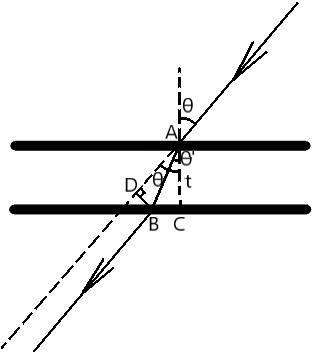
\includegraphics[scale = .8]{FigureofProblem1-4.png}
\caption{1-4题图}\label{FigureofProblem1-4}
\end{figure}
\section*{1-6}解:
如图\ref{FigureofProblem1-6},由于垂直入射,在第一个折射面上,光线不发生偏折,在第二个折射面上,由几何关系知,入射角$\theta_1 = \alpha$,根据斯涅耳定律,有
\[
n\sin\theta_1 = n\sin\alpha = \sin\theta_2
\]
又因为顶角$\alpha$很小,故解得
\[
\theta_2\approx n\alpha
\]
偏向角为
\[
\delta = \theta_2 - \alpha = (n - 1)\alpha
\]
\begin{figure}[h]
\centering
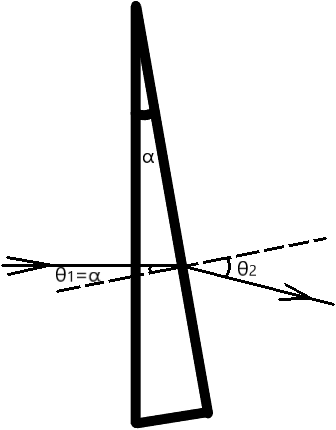
\includegraphics[scale = .6]{FigureofProblem1-6.png}
\caption{1-6题图}\label{FigureofProblem1-6}
\end{figure}
\section*{1-11}
\subsection*{(1)}答:
是。

设光线$1$以角度$\theta_1$由水入射空气,折射角为$\theta_2$,光线$2$ 以$\theta_1$由水入射玻璃,折射角为$\theta_3$,再以$\theta_3$由玻璃入射空气,折射角为$\theta_4$。对于光线$1$,根据斯涅耳定律,有
\[
n_{water}\sin\theta_1 = n_{air}\sin\theta_2
\]
对于光线$2$,在水--玻璃交界面上,根据斯涅尔定律,有
\[
n_{water}\sin\theta_1 = n_{glass}\sin\theta_3
\]
在玻璃--空气交界面上,根据斯涅耳定律,有
\[
n_{glass}\sin\theta_3 = n_{air}\sin\theta_4
\]
联立以上各式,得
\[
\sin\theta_2 = \sin\theta_4
\]
由于$0 < \theta_2,\theta_4 < 90^{\circ}$,因此
\[
\theta_2 = \theta_4
\]
两光线射到空气中还平行。
\subsection*{(2)}答:
若光线$1$发生全反射,则说明光线$1$的折射角“大于$90^{\circ}$”而不存在折射,根据(1)中的结论,光线$2$在玻璃--空气交界面上的折射角与之相等,也“大于$90^{\circ}$”,因此,光线$2$在玻璃-空气交界面上也不存在折射,无法进入空气。
\section*{1-13}证明:
在空气--玻璃芯交界面上,根据斯涅耳定律,有
\[
n_0\sin\theta_1 = n_1\sin\theta_1'
\]
当光线在纤维内恰好发生全反射时,在玻璃芯--外套交界面上,根据斯涅耳定律,有
\[
n_1\sin\theta_2 = n_2
\]
此外,考虑几何关系,角$\theta_1$和角$\theta_2$互余
\[
\theta_1 + \theta_2 = 90^{\circ}
\]
联立以上各式,解得能使光线在纤维内发生全反射的入射光束的最大孔径角$\theta_1$满足下式
\[
n_0\sin\theta_1 = \sqrt{n_1^2 - n_2^2}
\]
\section*{1-16}
\subsection*{(1)}解:
黄光的频率为
\[
\nu = \frac{c}{\lambda} = \frac{2.998\times10^8m/s}{589.3\times10^{-9}m} = 5.087\times10^{14}Hz
\]
\subsection*{(2)}解:
在折射率为$1.52$玻璃中,光速变为
\[
c' = \frac{c}{1.52}
\]
此时,黄光的波长为
\[
\lambda = \frac{c'}{\nu} = \frac{2.998\times10^8m/s}{1.52\times5.087\times10^{14}Hz} = 3.88\times10^{-7}m = 388nm
\]
\section*{1-18}
如表\ref{TableofProblem1-18}。
\begin{table}[ht]
\centering
\footnotesize
\begin{tabular}{| c | c | c | c | c | c |}
\hline
谱线 & \multicolumn{2}{| c |}{F线} && \multicolumn{2}{| c |}{D线}\\
\hline
介质 & 真空 & 水 && 真空 & 水\\
\hline
折射率$n$ & $1$ & $1.337$ && $1$ & $1.333$\\
\hline
波长$\lambda = \frac{c}{\nu}$ & $486.1nm$ & $363.5nm$ && $589.3nm$ & $442.1nm$\\
\hline
频率$\nu = \frac{c}{\lambda}$ & $6.167\times10^{14}Hz$ & $6.167\times10^{14}Hz$ && $5.087\times10^{14}Hz$ & $5.087\times10^{14}Hz$\\
\hline
光速$c' = \frac{c}{n}$ & $2.998\times10^8m/s$ & $2.242\times10^8m/s$ && $2.998\times10^8m/s$ & $2.249\times10^8m/s$ \\
\hline
\end{tabular}
\caption{1-18题表}\label{TableofProblem1-18}
\end{table}
\section*{1-19}证明:
如图\ref{FigureofProblem1-19},船沿$A_1A_n$方向行驶,船在水面上经过的每一点都可视为一个独立产生水波的波源,这些波纹的包络面就形成了圆锥形波前。设船在时间间隔$\Delta t$内由点$A_i$行驶到点$A_n$,行驶的距离$A_iA_n = v\Delta t$,在这段时间间隔内船在经过点$A_i$ 时产生的水波运动了距离$A_iB_i = ut$,在直角三角形$A_iA_nB_i$ 中,角$\angle A_iA_nB_i$ 即半顶角$\theta$ 满足
\[
\sin\theta = \sin\angle A_iA_nB_i = \frac{A_iB_i}{A_iA_n} = \frac{u\Delta t}{v\Delta t} = \frac{u}{v}
\]
当电子以大于介质中光速的速度在介质中做匀速运动,变化的电场产生磁场,变化的磁场产生电场,两者相互交替着向周围传播,因为电磁波在介质中的传播速度小于电子运动的速度,同理会产生类似的圆锥状的光波面,称为切连科夫辐射。
\begin{figure}%[h]
\centering
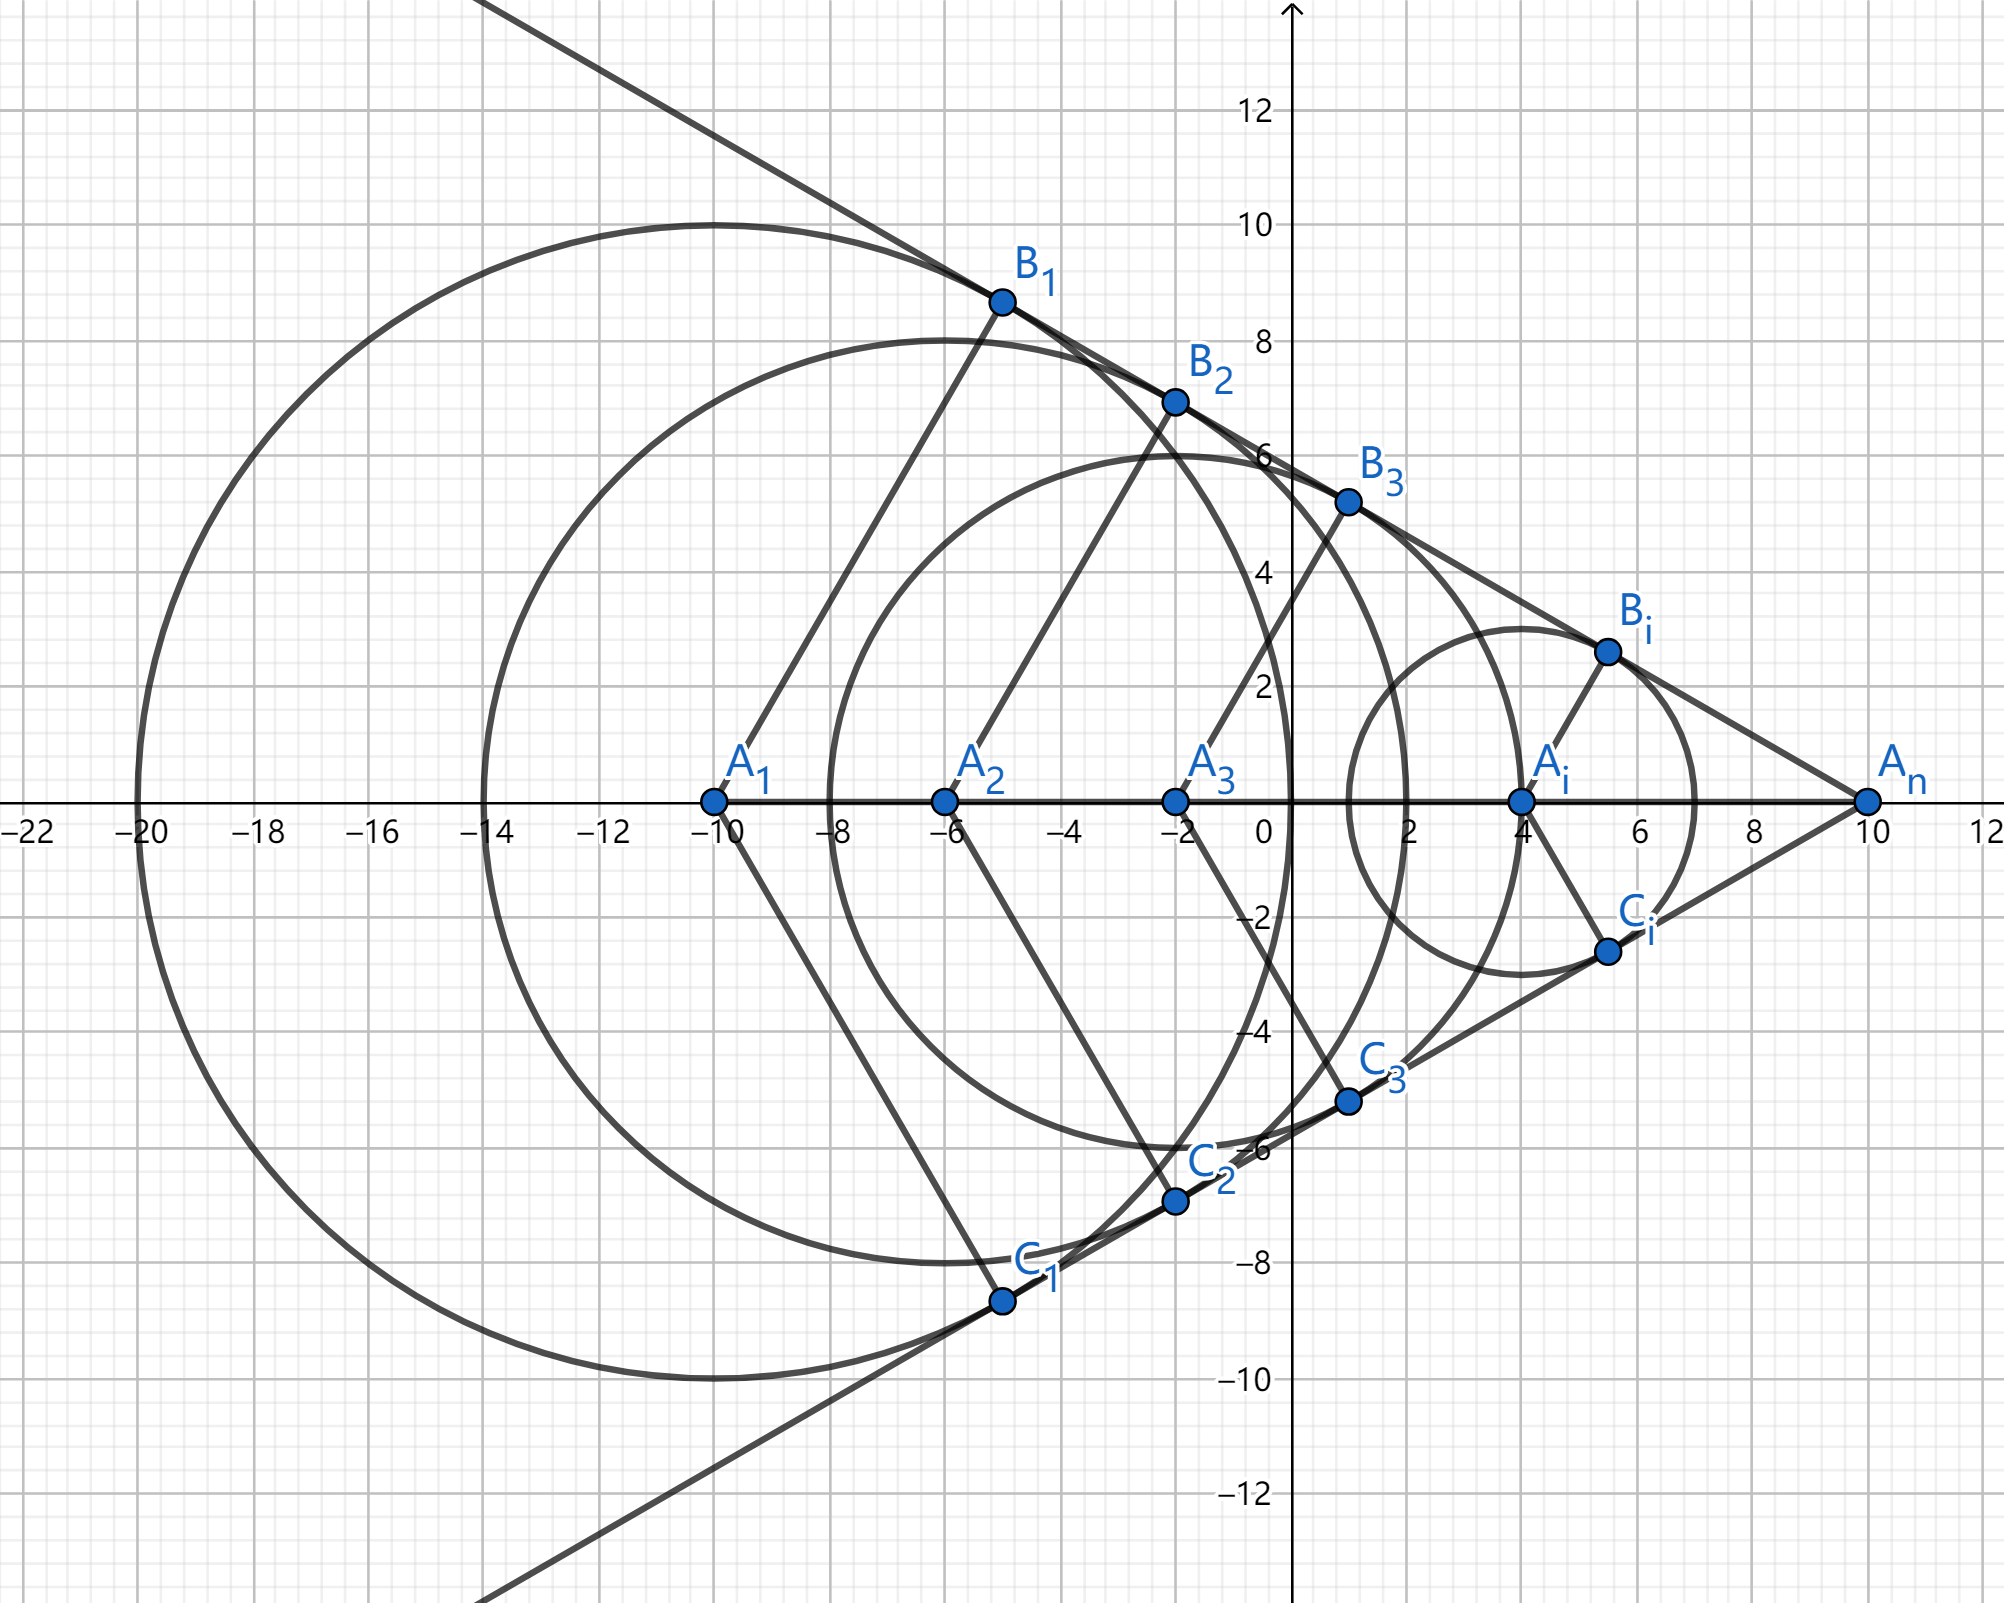
\includegraphics[scale = .15]{FigureofProblem1-19(tailored).png}
\caption{1-19题图}\label{FigureofProblem1-19}
\end{figure}
\section*{1-20}证明:
如图\ref{FigureofProblem1-20/21},过点$A_1$做$C_1B_n$的平行线与$B_iC_i$交于点$E_i$。
\begin{align*}
&\text{由对顶角定理,有}\angle A_1B_nE_i = \angle C_iB_iB_n\\
&\text{又由反射定律,有}\angle C_iB_iB_n = \angle A_iB_iA_1\\
&\therefore \angle A_1B_nE_i = \angle A_iB_iA_1\\
&\because \angle A_nA_1B_n + \angle A_1B_nA_n + \angle B_nA_nA_1 = 180^{\circ}\\
&\angle C_1B_nA_1 + \angle B_nA_1C_1 + \angle A_1C_1B_n = 180^{\circ}\\
&\text{波面}A_1A_n \perp \text{光线}A_nB_n\\
&\text{波面}B_nC_1 \perp \text{光线}C_1A_1\\
&\therefore \angle A_nA_1B_n = \angle C_1B_nA_1\\
&\because C_1B_n \parallel A_1E_i\\
&\therefore \angle C_1B_nA_1 = \angle E_iA_1B_n\\
&\text{在}\triangle A_1A_iB_i\text{和}\triangle A_1E_iD_i\text{中}\\
&\angle A_iA_1B_i = \angle E_iA_1B_i\\
&A_1B_i = A_1B_i\\
&\angle A_iB_iA_1 = \angle E_iB_iA_1\\
&\therefore \triangle A_1A_iB_i \cong \triangle A_1E_iB_i\\
&A_iB_i = E_iB_i\\
&\because A_1C_1 \parallel C_1E_1\\
&C_1C_i \parallel A_iE_i\\
&\text{光线}A_1C_1 \perp \text{波面}C_1B_n\\
&\therefore \text{四边形}A_1C_1C_iE_i\text{是矩形}\\
&\therefore A_1C_1 = C_iE_i = C_iB_iA_i\\
&\text{又}\because\text{入射光线和反射光线在同一介质中,折射率}n\text{相等}\\
&\therefore\text{光线}A_1C_1\text{和}A_iB_iC_i\text{光程相等}\\
&\therefore A_1C_1,A_2B_2C_2,A_3B_3C_3,\cdots,A_nB_n\text{光程相等}
\end{align*}
\section*{1-21}证明:
如图\ref{FigureofProblem1-20/21},由几何关系,有
\[
A_1B_n = \frac{A_1D_i}{\sin\angle A_1B_nD_1} = \frac{A_iB_i}{\sin\angle A_nA_iB_n} + \frac{B_iD_i}{\sin\angle A_1B_nD_1}
\]
根据斯涅尔定律,有
\[
n_1 \sin\angle A_1B_nC_1 = n_2 \sin\angle A_1B_nD_1
\]
\begin{align*}
&\therefore\text{光线}A_1D_1\text{的光程差} = n_1A_1D_1 = n_1A_iB_i + n_2B_iD_i = \text{光线}A_iB_iD_i\text{的光程差}\\
&\therefore\text{光线}A_1D_1,A_2B_2D_2,A_3B_3D_3,\cdots,A_nB_n\text{的光程相等}
\end{align*}
\begin{figure}%[h]
\centering
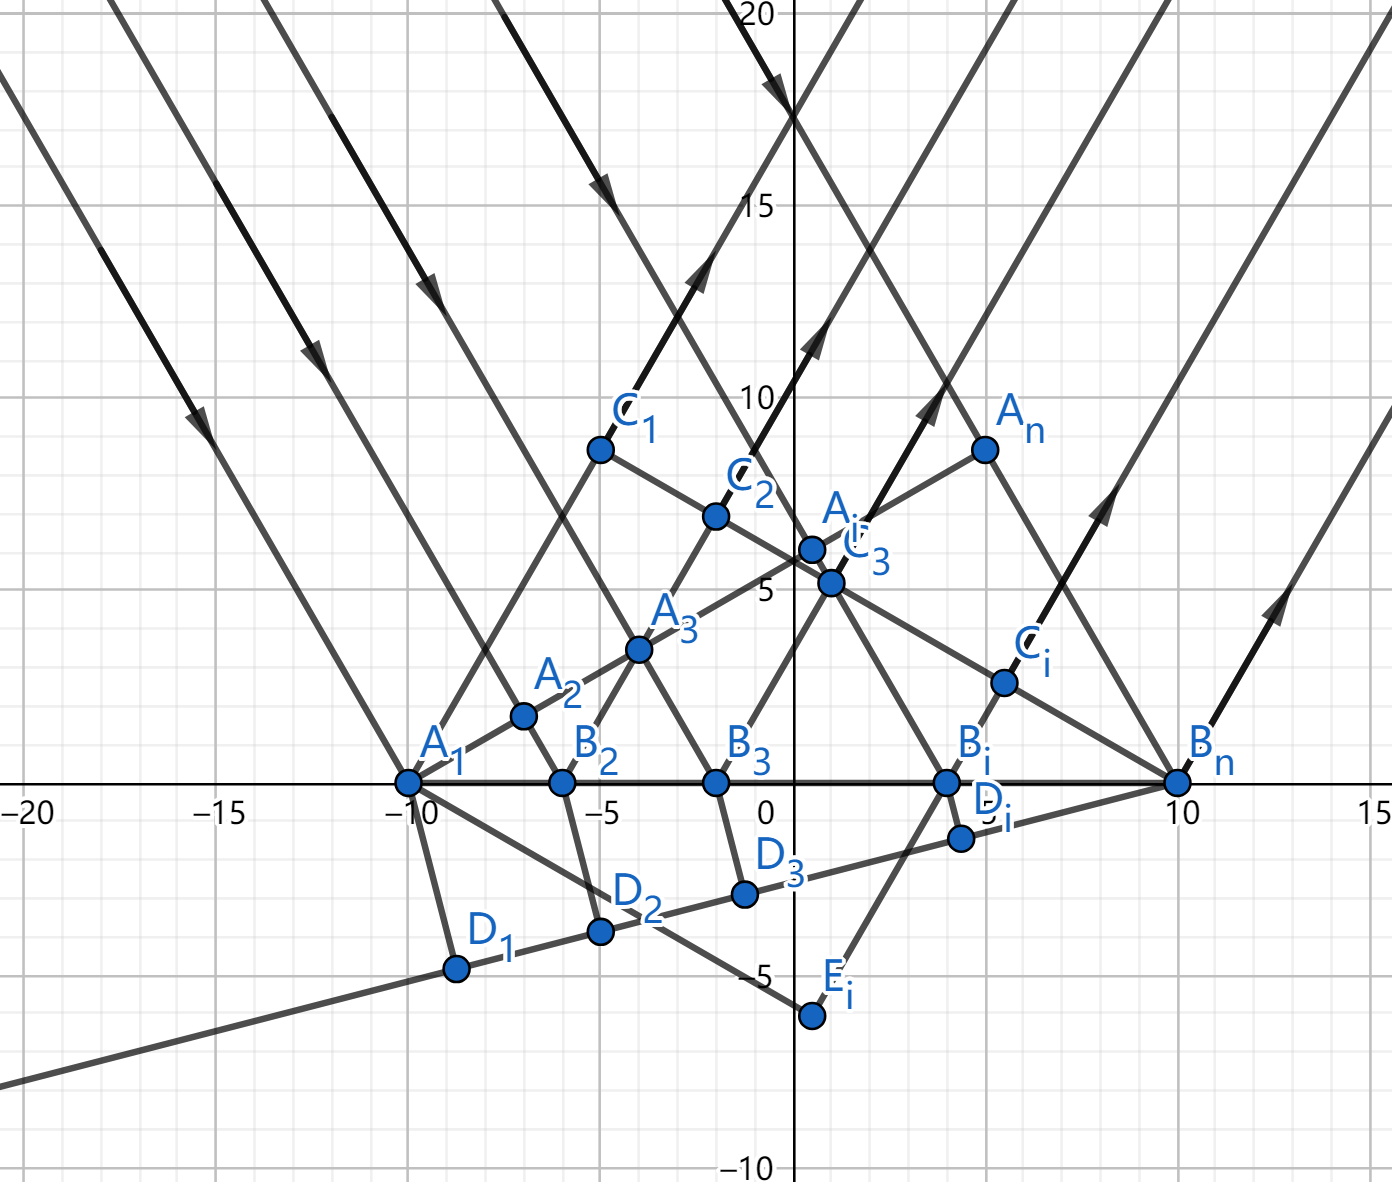
\includegraphics[scale = .3]{FigureofProblem1-20_21(tailored).png}
\caption{1-20/21题图}\label{FigureofProblem1-20/21}
\end{figure}
\end{document}